% Main article source. Compile with XeLaTeX twice.
% Both vector figures must be in the same directory.
\documentclass[11pt,a4paper]{article}
\usepackage[T1]{fontenc}
\usepackage[utf8]{inputenc}
\usepackage[a4paper,margin=1in]{geometry}
\usepackage[reqno]{amsmath}
\usepackage{amssymb,amsthm,mathtools}
\usepackage{graphicx}
\usepackage{microtype}
\usepackage[hidelinks]{hyperref}
\hypersetup{
  pdfauthor={Timofei Iuzhakov, Dmitry Vetrov},
  pdftitle={A proof of Cohn and Rajagopal's four-color density conjecture}
}

\newtheorem{theorem}{Theorem}[section]
\newtheorem{lemma}[theorem]{Lemma}
\newtheorem{proposition}[theorem]{Proposition}
\newtheorem{corollary}[theorem]{Corollary}
\theoremstyle{definition}
\newtheorem{definition}[theorem]{Definition}
\theoremstyle{remark}
\newtheorem{remark}[theorem]{Remark}

\newcommand{\R}{\mathbb{R}}
\newcommand{\Z}{\mathbb{Z}}
\newcommand{\N}{\mathbb{N}}
\DeclareMathOperator{\area}{area}
\DeclareMathOperator{\vol}{vol}
\DeclareMathOperator{\conv}{conv}
\DeclareMathOperator{\dist}{dist}
\DeclareMathOperator{\relint}{relint}

\title{A proof of Cohn and Rajagopal's four-color density conjecture}
\author{Timofei Iuzhakov \and Dmitry Vetrov}
\date{}

\begin{document}

\maketitle

\begin{abstract}
Consider a set of points in the Euclidean plane, each assigned a color in
$\Z/4\Z$. The colors are cyclically ordered as $0,1,2,3$. Colors are
adjacent if they are consecutive in this cycle, and opposite if they
differ by $2$. Any two distinct points of the same color must be at least
$\sqrt2$ apart. Points with adjacent colors must be at least $\sqrt5/2$
apart, and points with opposite colors at least $1$ apart. We prove that
every such configuration has upper radial point density at most $1$,
settling Conjecture~4.1 of Cohn and Rajagopal. We first establish a sharp
weighted cotangent inequality for colored triangles. For periodic
configurations, summing over a weak Delaunay triangulation gives the
density bound. The triangulation respects the periods and allows more
than three points on one circumcircle. Repeating finite patches after
removing boundary strips extends the bound to arbitrary configurations,
with an explicit error estimate. As a consequence, $D_5$ is optimal
within the family built from four translates of $D_3$ over a planar base,
even when the base has no ordinary density limit.
\end{abstract}

\noindent\textbf{2020 Mathematics Subject Classification.} 52C17, 52C15.

\noindent\textbf{Keywords.} sphere packing, colored point configurations, Delaunay triangulation,
cotangent inequality, upper density.


\section{The four-color density theorem}
\label{sec:introduction}

Cohn and Rajagopal associate certain five-dimensional sphere packings with
four-colored point configurations in the plane~\cite[Section~4.1]{CR}.
Their Conjecture~4.1 is the planar density estimate proved below.

We use the cyclic color set $\Z/4\Z$: colors differing by $\pm1$ are
\emph{adjacent}, and colors differing by $2$ are \emph{opposite}.
These terms refer to color labels, not to the positions of points.
The required minimum distances are $\sqrt2$ for equal colors,
$\sqrt5/2$ for adjacent colors, and $1$ for opposite colors.
For the proof, we use their squares, $2$, $5/4$, and $1$, as weights.

For $i,j\in\Z/4\Z$, define
\begin{equation}
\label{eq:weights}
\omega(i,j)=
\begin{cases}
2,&i=j,\\
1,&i-j\equiv2\pmod4,\\
\dfrac54,&i-j\equiv\pm1\pmod4.
\end{cases}
\end{equation}
A four-colored configuration is a pair $(C,c)$, where
$C\subset\R^2$ and $c:C\to\Z/4\Z$. The coloring need not use all four
colors. We use $|v|$ for the Euclidean norm of a vector and $|D|$ or
$\#D$ for the cardinality of a finite set.

\begin{definition}
\label{def:admissible}
A configuration $(C,c)$ is \emph{admissible} if
\begin{equation}
\label{eq:admissible}
|p-q|^2\geq\omega(c(p),c(q))
\qquad(p,q\in C,\ p\ne q).
\end{equation}
\end{definition}

For $r\geq0$, our ball notation is
\[
B_d(x,r)=\{y\in\R^d:|y-x|<r\},\qquad
\overline B_d(x,r)=\{y\in\R^d:|y-x|\leq r\}.
\]
For $r>0$, the closed ball is the closure of the open ball. At $r=0$,
the open ball is empty and the closed ball is $\{x\}$.
We omit the subscript when the dimension is clear.

Because $\omega\geq1$, every admissible configuration is $1$-separated:
any two distinct points are at distance at least $1$. We next prove local
finiteness, meaning that every bounded region contains only finitely many
points. Fix $r\geq0$ and a finite
subset $D\subset C\cap\overline B(0,r)$. The open disks of radius $1/2$
centered at the points of $D$ are pairwise disjoint and lie in
$B(0,r+1/2)$. Additivity and monotonicity of area give
\[
|D|\frac{\pi}{4}\leq\pi(r+1/2)^2,
\qquad |D|\leq4(r+1/2)^2.
\]
An infinite set contains finite subsets of arbitrarily large cardinality.
The displayed bound therefore forces $C\cap\overline B(0,r)$ to be finite.
Consequently the counting function
\[
N_C(r)=\#\{p\in C:|p|\leq r\}
\]
is finite for every $r\geq0$. For $r>0$, the ratio $N_C(r)/(\pi r^2)$ counts
points per unit area in the disk of radius $r$. Its limit superior as
$r\to\infty$ is the \emph{upper radial point density}; an ordinary limit
is not assumed to exist.
\begin{theorem}[Cohn--Rajagopal's Conjecture 4.1]
\label{thm:main}
Every admissible configuration $(C,c)$ satisfies
\begin{equation}
\label{eq:main-limsup}
\limsup_{r\to\infty}\frac{N_C(r)}{\pi r^2}\leq1.
\end{equation}
Equivalently, for every $\varepsilon>0$ there is $R\geq1$ such that
\begin{equation}
\label{eq:main-eventual}
N_C(r)\leq(1+\varepsilon)\pi r^2\qquad(r\geq R).
\end{equation}
The constant $1$ is attained.
\end{theorem}

Cohn and Rajagopal state their conjecture for infinite discrete
configurations. Here finite configurations are allowed, and discreteness
is a consequence of the distance conditions. On their intended infinite
class, \eqref{eq:main-limsup} is exactly
\cite[Conjecture~4.1]{CR}.

The proof starts with an inequality for a single colored triangle. An
individual cotangent may be negative, so the distance constraints cannot be
inserted into the triangle's area identity one edge at a time. We first
handle periodic configurations. A weak Delaunay triangulation makes the
sum of the two cotangents opposite each edge nonnegative. Pairing these
terms and summing over one period gives at least one unit of area per
point. The quotient torus records this sum with opposite sides of a
period square identified. Removing a boundary strip from a finite patch
then permits periodic repetition and proves the estimate without a
periodicity assumption.

The planar proof occupies Sections~\ref{sec:local}--\ref{sec:sharpness}.
Section~\ref{sec:local} proves the weighted cotangent inequality.
Section~\ref{sec:delaunay} constructs the required triangulation, and
Section~\ref{sec:global} uses it to prove the periodic density bound.
Sections~\ref{sec:periodization} and~\ref{sec:sharpness} remove periodicity
and prove sharpness, respectively.

Salmon~\cite[Theorem~26]{Salmon} proved that the
translation-invariant two-point colored linear program for this problem
has value strictly greater than~$1$. Thus that linear programming bound
cannot establish the conjectured density. The proof here uses a local
inequality for colored triangles and a Delaunay triangulation.

As a consequence, $D_5$ is optimal within the four-coset $D_3$-fibered
family of Cohn and Rajagopal. Section~\ref{sec:fibers} recalls this
construction after the planar proof; Appendix~\ref{app:density}
justifies the density transfer without assuming a density limit for the
base. This does not establish the global optimality of $D_5$ among all
five-dimensional sphere packings.

\section{A sharp weighted cotangent inequality}
\label{sec:local}

We seek an inequality involving only the colors and angles of a
triangle. No admissibility assumption is needed in this section's main
inequality; the distance bounds will enter the global sum in
Section~\ref{sec:global}.

Let $ABC$ be a nondegenerate Euclidean triangle with area $K>0$. We also
use $A,B,C$ for its angles. Write
\begin{equation}
\label{eq:squared-sides}
x=|B-C|^2,\qquad y=|C-A|^2,\qquad z=|A-B|^2,
\end{equation}
and attach to these sides the weights
\[
\alpha=\omega(c(B),c(C)),\quad
\beta=\omega(c(C),c(A)),\quad
\gamma=\omega(c(A),c(B)).
\]
Thus $\alpha,\beta,\gamma$ are the weights attached to the angles
$A,B,C$, respectively. To express the cotangents in terms of the squared
side lengths and area, put
\begin{equation}
\label{eq:heron}
H=2xy+2yz+2zx-x^2-y^2-z^2.
\end{equation}
If $u=B-A$ and $v=C-A$, then $z=|u|^2$, $y=|v|^2$, and
$x=y+z-2\langle u,v\rangle$. Substitution gives
\begin{equation}
\label{eq:heron-area}
H=4\bigl(|u|^2|v|^2-\langle u,v\rangle^2\bigr)=16K^2.
\end{equation}
The dot product and the area of the parallelogram give
\begin{equation}
\label{eq:cot-formulas}
\cot A=\frac{y+z-x}{4K},\qquad
\cot B=\frac{z+x-y}{4K},\qquad
\cot C=\frac{x+y-z}{4K}.
\end{equation}
Thus, on defining
\begin{equation}
\label{eq:marked-numerator}
N=\alpha(y+z-x)+\beta(z+x-y)+\gamma(x+y-z),
\end{equation}
we have
\begin{equation}
\label{eq:marked-quotient}
\alpha\cot A+\beta\cot B+\gamma\cot C=\frac{N}{4K}.
\end{equation}

\begin{lemma}[Color triples]
\label{lem:color-triples}
Up to simultaneous permutation of weights and opposite squared side
lengths, $(\alpha,\beta,\gamma)$ is one of
\begin{equation}
\label{eq:color-triples}
(2,2,2),\qquad(2,\tfrac54,\tfrac54),\qquad
(2,1,1),\qquad(\tfrac54,\tfrac54,1).
\end{equation}
\end{lemma}

\begin{proof}
If all three colors coincide, every weight is $2$. If precisely two
colors coincide, the side joining that pair has weight $2$. The remaining
color is either adjacent to both equal colors, giving the other two
weights $5/4$, or opposite to both, giving the other two weights $1$.
Finally, suppose that all three colors differ. Translating every color
by the same element of $\Z/4\Z$ does not change any weight. After such a
translation the three colors, without regard to order, are $0,1,2$.
Their pairs have weights $5/4,5/4,1$. These cases exhaust the possible
numbers of distinct colors and prove the list.
\end{proof}

\begin{theorem}[Weighted cotangent inequality]
\label{thm:triangle}
Every nondegenerate colored triangle satisfies
\begin{equation}
\label{eq:triangle-inequality}
\alpha\cot A+\beta\cot B+\gamma\cot C\geq2.
\end{equation}
Equality holds if and only if, up to simultaneous permutation, one of the
following holds for some $t>0$:
\begin{align}
\label{eq:equality-right}
(\alpha,\beta,\gamma)&=(2,1,1),&
(x,y,z)&=(2t,t,t),\\
\label{eq:equality-isosceles}
(\alpha,\beta,\gamma)&=(\tfrac54,\tfrac54,1),&
(x,y,z)&=(\tfrac54t,\tfrac54t,t).
\end{align}
\end{theorem}

\begin{proof}
By \eqref{eq:marked-quotient}, it suffices to prove $N\geq8K$.
We will compare their squares, using $H=16K^2$. First we show that
$N>0$, so that this comparison will imply the required inequality.
Collecting the coefficients of $x,y,z$ in
\eqref{eq:marked-numerator} gives

\begin{equation}
\label{eq:n-positive}
N=(-\alpha+\beta+\gamma)x
 +(\alpha-\beta+\gamma)y
 +(\alpha+\beta-\gamma)z.
\end{equation}

Every coefficient is nonnegative: for example,
$-\alpha+\beta+\gamma\geq-2+1+1=0$. The sum of the three
coefficients is $\alpha+\beta+\gamma>0$, so at least one coefficient is
positive. Nondegeneracy gives $x,y,z>0$, and therefore $N>0$.

We now compute $N^2-4H$ in each case of Lemma~\ref{lem:color-triples}.

\smallskip\noindent\emph{Case 1.} $(\alpha,\beta,\gamma)=(2,2,2)$.
Here $N=2(x+y+z)$, and
\begin{equation}
\label{eq:sos-222}
N^2-4H=4(x+y+z)^2-4H=8(x^2+y^2+z^2)>0.
\end{equation}

\smallskip\noindent\emph{Case 2.} $(\alpha,\beta,\gamma)=(2,\tfrac54,\tfrac54)$.
Here $N=x/2+2y+2z$. Expanding and completing squares gives
\begin{equation}
\label{eq:sos-255}
\begin{aligned}
N^2-4H
 &=\tfrac{17}{4}x^2+8y^2+8z^2-6x(y+z)\\
 &=4(y+z-\tfrac34x)^2+2x^2+4(y-z)^2>0.
\end{aligned}
\end{equation}

\smallskip\noindent\emph{Case 3.} $(\alpha,\beta,\gamma)=(2,1,1)$.
Here $N=2y+2z$, and
\begin{equation}
\label{eq:sos-211}
\begin{aligned}
N^2-4H
 &=4x^2+8y^2+8z^2-8x(y+z)\\
 &=4(x-y-z)^2+4(y-z)^2\geq0.
\end{aligned}
\end{equation}

\smallskip\noindent\emph{Case 4.} $(\alpha,\beta,\gamma)=(\tfrac54,\tfrac54,1)$.
Here $N=x+y+3z/2$, and
\begin{equation}
\label{eq:sos-551}
\begin{aligned}
N^2-4H
 &=5x^2+5y^2+\tfrac{25}{4}z^2-6xy-5z(x+y)\\
 &=(x+y-\tfrac52z)^2+4(x-y)^2\geq0.
\end{aligned}
\end{equation}

All four expressions are nonnegative. Since $H=16K^2$, this proves
$N^2\geq4H=(8K)^2$. Both $N$ and $8K$ are positive, so $N\geq8K$.
Dividing by $4K>0$ in \eqref{eq:marked-quotient} gives
\eqref{eq:triangle-inequality}.

Equality is equivalent to $N^2-4H=0$. Cases 1 and 2 are strict because
$x>0$. In Case 3 both squares must vanish, giving $y=z$ and $x=y+z$.
Writing $t=y>0$ gives \eqref{eq:equality-right}. In Case 4 both squares
must vanish, giving $x=y$ and $x+y=5z/2$. Writing $t=z>0$ gives
\eqref{eq:equality-isosceles}.

Conversely, these squared side lengths are realized, respectively, by
\[
(A,B,C)=\bigl((0,0),(\sqrt t,0),(0,\sqrt t)\bigr)
\]
and by
\[
(A,B,C)=\bigl((-\sqrt t/2,0),(\sqrt t/2,0),(0,\sqrt t)\bigr).
\]
Both triangles have area $t/2>0$. With the stated weights, their
corresponding sums of squares vanish; reversing the preceding positive
division proves equality.
\end{proof}

In \eqref{eq:equality-right}, $B,C$ have the same color and $A$ has their
opposite color. In \eqref{eq:equality-isosceles}, $A,B$ have opposite colors
and $C$ is adjacent to both. The inequality itself imposes no lower bound
on $t$, since angles are invariant under scaling.

\begin{corollary}
\label{cor:triangle-scale}
If the vertices of an equality triangle belong to an admissible
configuration, then $t\geq1$ and the triangle has area $t/2$.
At $t=1$ its side lengths are one of the two triples
\begin{equation}
\label{eq:two-tiles}
\Delta_1:\quad(\tfrac{\sqrt5}{2},\tfrac{\sqrt5}{2},1),
\qquad
\Delta_2:\quad(1,1,\sqrt2).
\end{equation}
Both triangles have area $1/2$.
\end{corollary}

\begin{proof}
In \eqref{eq:equality-right}, admissibility gives $2t\geq2$ and $t\geq1$.
In \eqref{eq:equality-isosceles}, it gives $5t/4\geq5/4$ and $t\geq1$.
Substitution into \eqref{eq:heron-area} gives $K=t/2$ in both cases.
\end{proof}

These are precisely the two triangle shapes used by Cohn and
Rajagopal~\cite[Section~4.1]{CR} to construct four-colored planar configurations of point density~$1$.
Figure~\ref{fig:triangles} shows them at their minimum admissible scale.

\begin{figure}[!htbp]
\centering
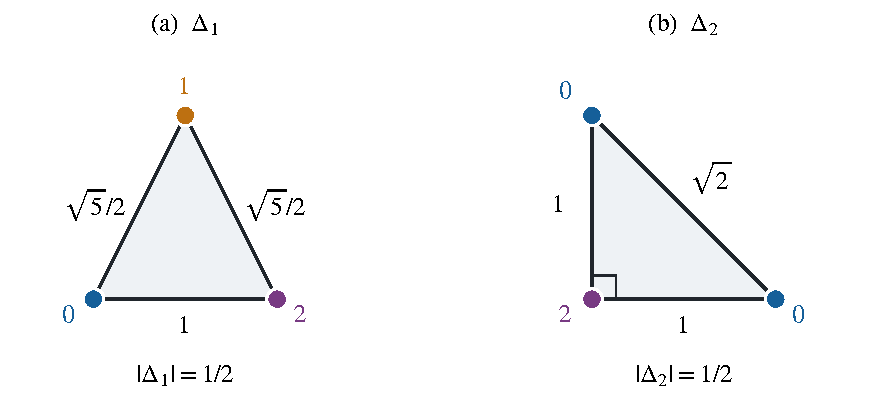
\includegraphics[width=.86\linewidth]{equality_triangles.pdf}
\caption{The two minimally scaled equality triangles. Vertex numerals
are colors in $\Z/4\Z$. In $\Delta_2$, the endpoints of the side of
length $\sqrt2$ have the same color; in $\Delta_1$, the endpoints of
the side of length $1$ have opposite colors. This is a local equality
statement, not a classification of all configurations of density $1$.}
\label{fig:triangles}
\end{figure}

\section{A periodic weak Delaunay triangulation}
\label{sec:delaunay}

Fix $L>0$ and put $\Lambda=L\Z^2$. Let $S\subset\R^2$ be a nonempty
finite set such that no two distinct elements of $S$ differ by an element
of $\Lambda$. The corresponding periodic point set is
\[
X=S+\Lambda.
\]
Two points lie in the same \emph{orbit} if one is a translate of the other
by an element of $\Lambda$. Thus $S$ contains exactly one representative
of each point orbit. Assume that the coloring of $S$ repeats under these
translations and that $X$ is admissible. Write $V=|S|$.
The same terminology will be used for edge and face orbits. A
$\Lambda$-equivariant triangulation is one preserved by every translation
in $\Lambda$.

A straight-line triangulation is called \emph{weakly Delaunay} if, for
each edge, the sum of the two opposite angles is at most $\pi$. Equality
is allowed. We construct such a triangulation from polygons whose vertices
lie on circles with no points of $X$ in their interiors; additional
points on the circles are allowed. The following proposition supplies the triangulation and
the quotient identities needed for the cotangent sum in
Section~\ref{sec:global}.
Delaunay tessellations and their cotangent weights are standard; see
Bobenko and Springborn~\cite{BS}. We give the periodic planar construction explicitly, including the case
of more than three points on one empty circle and the identifications
arising from periodicity.

\begin{proposition}
\label{prop:triangulation}
There is a locally finite, straight-line, $\Lambda$-equivariant weak
Delaunay triangulation $\mathcal D$ of $\R^2$ with the following properties:
\begin{enumerate}
\item[(i)] its vertices are exactly $X$, and all triangular faces are
nondegenerate;
\item[(ii)] the faces cover $\R^2$, have pairwise disjoint interiors, and
meet along full edges or vertices;
\item[(iii)] there are finitely many vertex, edge, and face orbits;
\item[(iv)] if $F$ is the number of face orbits, then
\begin{equation}
\label{eq:torus-identities}
\sum_{f\in\mathcal D/\Lambda}\area(f)=L^2,
\qquad F=2V.
\end{equation}
\end{enumerate}
In the sum in \eqref{eq:torus-identities}, one representative of each face
orbit is used.
\end{proposition}

\begin{proof}
Steps~1--3 construct a locally finite Delaunay polygonal decomposition.
Step~4 triangulates its polygons, and Step~5 proves the quotient
identities. Throughout, the points remain fixed; in particular, we do not perturb
points that lie on a common circle.

\smallskip\noindent
\emph{Step 1: separation, covering radius, and Voronoi cells.}
Admissibility makes $X$ $1$-separated. Choose $s_0\in S$. Rounding both
coordinates of $(z-s_0)/L$ to nearest integers shows that every
$z\in\R^2$ lies within distance
\[
R_0=\frac{L}{\sqrt2}
\]
of a point of $s_0+\Lambda\subset X$: the two coordinate errors are at
most $L/2$, so their squared sum is at most $L^2/2$. Thus $R_0$ is a covering radius: every location in the plane is within
$R_0$ of $X$. We call the points of $X$ \emph{sites}. A nearest site
exists for every $z$. Indeed, choose any $x_0\in X$ and put
$D=|z-x_0|$. The set $X\cap\overline B(z,D)$ is finite and nonempty,
so the distances to its points have a minimum. Every omitted point has
distance greater than $D$, and hence cannot decrease that minimum.

For $x\in X$, its Voronoi cell consists of the locations for which $x$
is a nearest site:
\[
\mathcal V_x=\{z:|z-x|\leq|z-y|\text{ for every }y\in X\}.
\]
Squaring and cancelling $|z|^2$ rewrites each comparison as
\[
2z\cdot(y-x)\leq |y|^2-|x|^2.
\]
Thus $\mathcal V_x$ is closed and convex. If $|z-x|<1/2$ and $y\ne x$,
then $|z-y|\geq |x-y|-|z-x|\geq1-|z-x|>|z-x|$.
Consequently the open disk $B(x,1/2)$ is contained in $\mathcal V_x$,
and hence in its interior. The comparisons with
$x\pm(L,0)$ and $x\pm(0,L)$ imply
\begin{equation}
\label{eq:voronoi-square}
\mathcal V_x\subset x+[-L/2,L/2]^2
\subset\overline B(x,R_0).
\end{equation}
Let $Y_x=X\cap\overline B(x,2R_0)$. This is finite and contains those four
translates. A point satisfying the comparisons with $Y_x$ already lies
in the square in \eqref{eq:voronoi-square}. For any omitted site $y$, it
therefore satisfies
\[
|z-y|\geq|x-y|-|z-x|>R_0\geq|z-x|.
\]
All omitted inequalities are redundant, so $\mathcal V_x$ is a compact
convex polygon cut out by finitely many half-planes.

The cells cover the plane because nearest sites exist. If $x\ne y$, then
\[
\mathcal V_x\cap\mathcal V_y
=\mathcal V_x\cap\{z:|z-x|=|z-y|\}.
\]
The equality holds because a point of $\mathcal V_x$ equidistant from
$x$ and $y$ also satisfies every defining comparison for
$\mathcal V_y$. The bisector is a supporting line whenever this
intersection is nonempty. Thus the intersection is a face of each cell:
a full side or a vertex. Finally, a cell meeting
a compact set $K$ has its site in the closed $R_0$-neighborhood of $K$.
There are only finitely many such sites. The Voronoi cells are therefore
locally finite, and translation by $\lambda\in\Lambda$ sends
$\mathcal V_x$ to $\mathcal V_{x+\lambda}$.

\smallskip\noindent
\emph{Step 2: constructing Delaunay cells from nearest sites.}
At each location, we take the convex hull of all nearest sites. For
$u\in\R^2$, define
\[
d(u)=\dist(u,X),\qquad
A(u)=\{x\in X:|u-x|=d(u)\},\qquad
P(u)=\conv A(u).
\]
Here $\conv$ denotes the convex hull, and the members of $A(u)$ are
called the \emph{active sites} at $u$. The set $A(u)$ is finite and
nonempty. All its points lie on the circle
with center $u$ and radius $d(u)\leq R_0$, and the open disk bounded by
that circle contains no point of $X$. When $d(u)=0$, the active set is a
singleton.

To prove that these cells cover the plane, fix $z\in\R^2$. We will find
a center $u$ whose cell contains $z$ by maximizing the following
auxiliary function:
\begin{equation}
\label{eq:variational}
\Phi_z(u)=d(u)^2-|u-z|^2
=\min_{x\in X}\bigl(|u-x|^2-|u-z|^2\bigr).
\end{equation}
The distance function is $1$-Lipschitz, since the triangle inequality
gives $d(u)\leq |u-v|+d(v)$ and the reverse inequality follows by
interchanging $u,v$. Hence $\Phi_z$ is continuous. Moreover,
\[
\Phi_z(u)\leq R_0^2-|u-z|^2\longrightarrow-\infty
\qquad(|u|\to\infty).
\]
Choose a closed ball outside which $\Phi_z(u)<\Phi_z(z)$.
On that compact ball the continuous function attains a maximum, and
this maximum is also global. Denote a maximizing point by $u_0$.

Suppose that $z\notin P(u_0)$. We will move $u_0$ slightly in a direction
that increases every active term, contradicting maximality. By compactness choose
$p\in P(u_0)$ minimizing $|z-p|$, and put $h=z-p\ne0$.
For $x\in P(u_0)$ and $0\leq s\leq1$, convexity places
$p+s(x-p)$ in $P(u_0)$. Minimality of $p$ gives
\[
|h-s(x-p)|^2\geq |h|^2.
\]
For $s>0$, expansion and division by $s$ give
$-2h\cdot(x-p)+s|x-p|^2\geq0$. Letting $s$ decrease to zero shows
$h\cdot(x-p)\leq0$. It follows that
\begin{equation}
\label{eq:projection-direction}
h\cdot(z-x)=|h|^2+h\cdot(p-x)\geq|h|^2
\qquad(x\in A(u_0)).
\end{equation}
Each function in the minimum in \eqref{eq:variational} is affine in $u$.
For an active site, \eqref{eq:projection-direction} implies
\[
|u_0+th-x|^2-|u_0+th-z|^2
\geq\Phi_z(u_0)+2t|h|^2.
\]
We must also control sites that were not active at $u_0$. For
$0\leq t\leq1$, every nearest site to $u_0+th$ has distance
at most $R_0$ from that point, and therefore lies in the fixed finite set
\[
Y=X\cap\overline B(u_0,R_0+|h|).
\]
For each inactive site $x\in Y\setminus A(u_0)$ put
\[
\delta_x=|u_0-x|^2-|u_0-z|^2-\Phi_z(u_0)>0,
\qquad b_x=2h\cdot(z-x).
\]
Its value in the affine minimum at $u_0+th$ is exactly
$\Phi_z(u_0)+\delta_x+tb_x$. Choose $0<t\leq1$ so small that
$t|b_x|<\delta_x/2$ for every inactive site; only finitely many
conditions occur. If there are no inactive sites, take any $0<t\leq1$.
Every inactive value is then greater than
$\Phi_z(u_0)+\delta_x/2$, while every active value is at least
$\Phi_z(u_0)+2t|h|^2$. Every site that can attain the minimum belongs
to $Y$. Hence $\Phi_z(u_0+th)>\Phi_z(u_0)$, contradicting maximality.
We conclude that $z\in P(u_0)$, which proves the covering assertion.

The converse will be used to prove that cells meet along common faces.
Suppose
$q=\sum_{x\in A(u)}\lambda_xx\in P(u)$, where $\lambda_x\geq0$ and
$\sum_x\lambda_x=1$. For every $v\in\R^2$,
\begin{align}
\label{eq:variational-converse}
\Phi_q(v)
&\leq\sum_x\lambda_x\bigl(|v-x|^2-|v-q|^2\bigr)\notag\\
&=\sum_x\lambda_x|x|^2-|q|^2
=\Phi_q(u).
\end{align}
For the middle equality, expand both squares: the coefficient of $v$
is $-2v\cdot(\sum_x\lambda_xx-q)=0$, and
$\sum_x\lambda_x=1$. For each $x\in A(u)$, the quantity
$|u-x|^2-|u-q|^2$ equals $\Phi_q(u)$ because $x$ is a nearest site to $u$.
Their weighted average has the same value, since the weights sum to $1$.
This proves the final equality, and shows that $u$ maximizes
$\Phi_q$ whenever $q\in P(u)$.

\smallskip\noindent
\emph{Step 3: common faces, local finiteness, and maximal cells.}
We use faces in the following elementary sense. The whole cell is a
face. A proper nonempty face of a polygon is a full side or a vertex.
For a segment, the proper nonempty faces are its endpoints. Such a proper
face is cut out by a supporting line.

In particular, suppose an interior point of a segment in a convex cell
belongs to a face. Then both endpoints belong to that face.
For a proper face, choose an affine function that is nonnegative on the
cell and whose zero set within the cell is that face. Its value at the
interior point is a convex combination of the endpoint values, with both
coefficients positive. Since this value is zero, both endpoint values
must be zero. The same assertion is immediate for the whole cell.

We now show that the intersection of two cells is a face of each.
Let $C=P(u)\cap P(v)$ be nonempty and choose $q\in\relint C$.
Here relative interior means interior within the affine hull, so the
relative interior of a singleton is the singleton itself. Let $F_u$
be the smallest face of $P(u)$ containing $q$. The point $q$ lies in
$\relint F_u$: it is either a vertex, an interior point of a side, or
an interior point of the cell in its affine hull.

We need to express $q$ as a convex combination that uses every vertex
of $F_u$ with a strictly positive coefficient. Write these vertices as
$x_1,\ldots,x_m$, and put
$b=m^{-1}\sum_i x_i$. For sufficiently small $\eta\in(0,1)$,
\[
q'=\frac{q-\eta b}{1-\eta}\in F_u,
\]
because $q\in\relint F_u$ and $q'$ approaches $q$ within the affine hull
of $F_u$ as $\eta\downarrow0$.
Write $q'=\sum_i\mu_i x_i$ with $\mu_i\geq0$ and
$\sum_i\mu_i=1$. Then
\[
q=\sum_{i=1}^m\lambda_i x_i,
\qquad \lambda_i=\frac\eta m+(1-\eta)\mu_i>0,
\qquad\sum_i\lambda_i=1.
\]
This also covers a singleton face, with $m=1$.
Each $x_i$ is a vertex of the convex hull of the finite set $A(u)$,
and hence belongs to $A(u)$.

Both $u$ and $v$ maximize $\Phi_q$, since $q$ belongs to both cells.
Using the positive combination above in
\eqref{eq:variational-converse} therefore gives
\[
\Phi_q(v)=\sum_i\lambda_i
\bigl(|v-x_i|^2-|v-q|^2\bigr).
\]
Each value $|v-x_i|^2-|v-q|^2$ is at least $\Phi_q(v)$.
Their weighted average equals $\Phi_q(v)$, and the positive weights sum
to $1$. Therefore every one of these values equals $\Phi_q(v)$.
Hence every $x_i$ is a nearest site to $v$: $x_i\in A(v)$. Taking convex hulls yields $F_u\subset P(v)$.

We also have $C\subset F_u$. To see this directly, take any $y\in C$.
If $y=q$, then $y\in F_u$. Otherwise, relative interior gives
$y'=q+\varepsilon(q-y)\in C$ for sufficiently small $\varepsilon>0$.
The identity
$q=\frac{\varepsilon}{1+\varepsilon}y+
\frac1{1+\varepsilon}y'$ places $q$ in the interior of the segment
joining $y$ and $y'$. Both endpoints lie in $P(u)$, and the face property
just explained forces both to belong to $F_u$. Thus $C=F_u$. Reversing $u,v$ shows
that a nonempty intersection is a face of both cells. In particular,
distinct two-dimensional cells have disjoint interiors.

Before passing to maximal cells, we verify local finiteness of the
\emph{whole} family, identifying repeated copies of the same geometric
cell. If $P(u)$ meets a compact set $K$, choose $z\in P(u)\cap K$.
The inclusion $A(u)\subset\overline B(u,R_0)$ and convexity of that
ball imply $|z-u|\leq R_0$. For $x\in A(u)$,
$|x-z|\leq |x-u|+|u-z|\leq2R_0$. Every point of $A(u)$ thus lies in
\[
X\cap K_{2R_0},
\]
where $K_{2R_0}$ is the closed $2R_0$-neighborhood of $K$. This is a fixed
finite set. Hence all cells meeting $K$ are convex hulls of subsets of one
finite set, and there are only finitely many of them. This argument also
covers zero- and one-dimensional cells.

Every cell is contained in a maximal cell: fix one of its points; only
finitely many cells contain that point.

Every maximal cell is
two-dimensional. Otherwise, take a relative-interior point $q$ of a
maximal cell $P$. Any other cell containing $q$ intersects $P$ in a face containing $q$.
Since $q$ is in the relative interior of $P$, this face is $P$ itself.
Thus the other cell contains $P$ and equals $P$ by maximality. Choose a compact closed ball about $q$. Only finitely many cells meet
it, and none except $P$ contains $q$. Each of the other cells is closed
and has positive distance from $q$. A smaller open ball about $q$,
contained in the first ball and with radius smaller than all these
finitely many distances, meets only $P$. If there are no other cells,
any smaller radius suffices. Since all cells cover the plane, that open
ball must lie in $P$. This is impossible when $\dim P<2$.

The maximal cells therefore form a locally finite covering by convex
cyclic polygons meeting along common faces. Their vertex set is exactly
$X$. Every vertex belongs to $X$ because the cells are convex hulls of
finite subsets of $X$. Conversely, for $x\in X$ we have $P(x)=\{x\}$.
This singleton lies in a maximal cell, and the common-face property makes
it a vertex of that cell. No point of $X$ lies in the relative interior of a Delaunay edge.
Indeed, if the edge has endpoints $a,b$ on the empty circle with center
$u$ and radius $r>0$, then for $0<t<1$,
\[
|(1-t)a+tb-u|^2=r^2-t(1-t)|a-b|^2<r^2.
\]
An interior point of the edge would therefore be inside the empty disk.

Translation by $\lambda\in\Lambda$ sends $A(u)$ to $A(u+\lambda)$ and
$P(u)$ to $P(u+\lambda)$. The polygonal decomposition is therefore
$\Lambda$-equivariant. Each maximal cell has at least three active
points, so its circle has positive radius and is uniquely determined by
its vertices.

\smallskip\noindent
\emph{Step 4: triangulation and the weak Delaunay condition.}
In each maximal cell, choose the vertex whose displacement from the
circumcenter is lexicographically least: compare first coordinates, then
second coordinates in case of a tie. This choice is unique because
there are finitely many distinct displacement vectors and lexicographic
order is a total order. Label the polygon vertices cyclically as
$v_0,v_1,\ldots,v_{m-1}$, starting with the chosen vertex. Draw the
diagonals from $v_0$ and take the triangles
\[
\conv\{v_0,v_i,v_{i+1}\},\qquad 1\leq i\leq m-2.
\]
Convexity puts every diagonal in the polygon. The successive rays from $v_0$ divide the polygon into the indicated
triangular sectors. To see this, take a ray from $v_0$ through an interior
point. Unless it passes through another vertex, it exits through exactly
one side of the chain $v_1,v_2,\ldots,v_{m-1}$. The portions of the exceptional rays inside the polygon are the inserted
diagonals. These diagonals form the common boundaries of successive sectors.
Thus these triangles cover the polygon and have disjoint interiors. No three distinct points of a circle are
collinear, so every triangle is nondegenerate.

Translations preserve the circumcenter displacements, the chosen
vertex, and this fan of diagonals. The construction is therefore
$\Lambda$-equivariant. It leaves every polygon boundary unchanged,
so triangulations of neighboring polygons agree along their common
faces. It introduces no vertices. Finally, a compact set meets only
finitely many original polygons, each subdivided into finitely many
triangles. The resulting triangulation is locally finite and has
vertex set exactly $X$.

Every resulting triangle has an empty open circumdisk: its circumcircle
is the circle of the original polygon. We verify the required angle
condition explicitly. First, every edge in the plane has exactly one incident triangle on
either side. Choose a point in the relative
interior of the edge. By local finiteness, a sufficiently small disk
about that point avoids all vertices and all edges not containing the
point. Coverage supplies an incident triangle on either side. Two on
the same side would have overlapping interiors near that point, which
is impossible. Thus, if the common edge is $AB$ and the opposite
vertices are $C,D$, those vertices lie on opposite sides of its line.
Choose coordinates
\[
A=(0,0),\quad B=(\ell,0),\quad C=(c,h),\quad D=(d,-k),
\qquad \ell,h,k>0.
\]
Put $\alpha=\angle ACB$ and $\beta=\angle ADB$. The dot-product
formula gives
\[
\cot\alpha=\frac{c^2-\ell c+h^2}{\ell h},
\qquad
\cot\beta=\frac{d^2-\ell d+k^2}{\ell k}.
\]
The circle through $A,B,C$ has equation
\[
x^2+y^2-\ell x-\ell(\cot\alpha)y=0.
\]
Completing the squares writes the left side as
\[
(x-\ell/2)^2+(y-\ell\cot\alpha/2)^2
-\frac{\ell^2}{4}(1+\cot^2\alpha).
\]
Its sign is therefore nonnegative on and outside the circle. The
empty-disk property places the site $D$ in that region, so evaluation
at $(d,-k)$ gives
\[
0\leq d^2+k^2-\ell d+\ell k\cot\alpha
=\ell k(\cot\alpha+\cot\beta).
\]
As both angles lie in $(0,\pi)$,
\[
\cot\alpha+\cot\beta
=\frac{\sin(\alpha+\beta)}{\sin\alpha\sin\beta}\geq0
\]
implies $\alpha+\beta\leq\pi$: the sum lies in $(0,2\pi)$, and
sine is negative on $(\pi,2\pi)$. For an inserted diagonal, all four
vertices lie on one circle and equality holds. Thus the triangulation is
weakly Delaunay, including the cocircular cases.

\smallskip\noindent
\emph{Step 5: area and incidence counts over one period.}
We now count one representative of each translation orbit. Equivalently,
we work on the quotient torus $\R^2/\Lambda$, obtained by identifying
opposite sides of a period square. A \emph{lift} is an actual point, edge,
or triangle in the plane representing an element of this quotient.
Let $Q=[0,L)^2$. Local finiteness implies that its compact closure meets
only finitely many triangles and edges. Every orbit has a representative
meeting that closure, so there are finitely many face and edge orbits.
A bounded edge or triangle is preserved only by the zero translation
(in group-action terminology, its translational stabilizer is trivial).
Indeed, if translation by $\lambda$ preserved it, all translates
$p+n\lambda$ of any one of its points would belong to it for every
integer $n$, contradicting boundedness unless $\lambda=0$.

The barycenter of a triangle is the average of its three vertices.
Translating a triangle translates its barycenter by the same vector.
Every point has exactly one translate in the half-open fundamental
square $Q$. Hence each face orbit has a unique representative whose
barycenter lies in $Q$.

For each such representative $T$, the sets
$T\cap(Q-\lambda)$, $\lambda\in\Lambda$, partition $T$; boundedness
implies that only finitely many have nonzero area. Translation by
$\lambda$ takes each piece to $(T+\lambda)\cap Q$ without changing
its area. Thus
\begin{align*}
\sum_{[T]\in\mathcal D/\Lambda}\area(T)
&=\sum_{[T]}\sum_{\lambda\in\Lambda}
   \area\bigl(T\cap(Q-\lambda)\bigr)\\
&=\sum_{[T]}\sum_{\lambda\in\Lambda}
   \area\bigl((T+\lambda)\cap Q\bigr)\\
&=\area(Q)=L^2.
\end{align*}
In the last equality, every lifted triangle occurs exactly once, the
triangles cover $Q$, and overlaps are contained in their edges. Only
finitely many triangles meet $\overline Q$, and their edges have area
zero, so there is no area overcounting.

To count angles, use incidences $(T,p)$ with $p$ a vertex of the lifted
triangle $T$. Translation acts on both entries. A face representative
has three different incidence orbits: an identification between two of
its corners would require a translation stabilizing $T$, and hence the
zero translation. Consequently the sum of the angles over all incidence
orbits is $\pi F$.

Alternatively, fix one lift $p$ of each vertex orbit. Every incidence orbit above that vertex orbit has exactly one
representative whose vertex is $p$. The required translation exists by
the definition of an orbit. It is unique because the action on points
is free.

Only finitely many triangles meet $p$. Choose a sufficiently small circle about $p$ so
that it meets no nonincident triangle and crosses only the two sides
through $p$ of each incident triangle. Such a choice is possible by
local finiteness, closedness, and the positive distances from $p$ to the
opposite sides. The sectors cut out arcs that cover the circle and overlap only at their
endpoints. Hence their angles sum to $2\pi$. There are $V$ vertex orbits. The same incidence
sum is therefore $2\pi V$, giving
\[
\pi F=2\pi V,\qquad F=2V.
\]
If several corners of a quotient face belong to the same vertex orbit,
they are still different incidence orbits and are counted separately.

Finally, use side incidences $(T,e)$, where $e$ is an edge of $T$.
A face representative contributes three different incidence orbits
because it has trivial translational stabilizer. For a fixed edge
representative, each incidence orbit has a unique lift incident to
that edge, since the edge also has trivial stabilizer. There are
exactly two such lifted incidences, one on each side, as proved in
Step~4. Thus
\[
3F=2E,
\]
where $E$ is the number of edge orbits. More generally, any
translation-invariant sum over face-side incidences can be regrouped
into the two contributions at each edge orbit. This is the precise
pairing used below. Loops, multiple edges, or identified corners in the
quotient do not change any of these incidence counts.
\end{proof}

\section{The global cotangent sum}
\label{sec:global}

We now combine the local inequality with the periodic triangulation.
The area identity below involves squared edge lengths. We first pair
the two terms at each edge, then use admissibility to replace these
lengths by color weights.

For a triangular face $f$ and one of its edges $e$, let
$\theta_{f,e}\in(0,\pi)$ be the opposite angle.

\begin{lemma}[Cotangent area identity]
\label{lem:area-identity}
Every nondegenerate Euclidean triangle of area $K_f$ satisfies
\begin{equation}
\label{eq:area-identity}
4K_f=\sum_{e\subset f}|e|^2\cot\theta_{f,e}.
\end{equation}
\end{lemma}

\begin{proof}
Substituting \eqref{eq:cot-formulas}, the numerator of the sum is
\[
x(y+z-x)+y(z+x-y)+z(x+y-z)=H=16K_f^2.
\]
Division by $4K_f$ proves the identity.
\end{proof}

\begin{lemma}[Paired Delaunay sign]
\label{lem:paired-sign}
If $\alpha_e,\beta_e$ are the angles opposite an edge in the two adjacent
triangles of a weak Delaunay triangulation, then
\begin{equation}
\label{eq:paired-sign}
\cot\alpha_e+\cot\beta_e\geq0.
\end{equation}
\end{lemma}

\begin{proof}
Both angles lie in $(0,\pi)$ and their sum is at most $\pi$. Therefore
\[
\cot\alpha_e+\cot\beta_e
=\frac{\sin(\alpha_e+\beta_e)}{\sin\alpha_e\sin\beta_e}\geq0.
\]
For four cocircular vertices, the numerator is zero.
\end{proof}

Figure~\ref{fig:cotangent} illustrates the pairing at a common edge.

\begin{figure}[tbp]
\centering
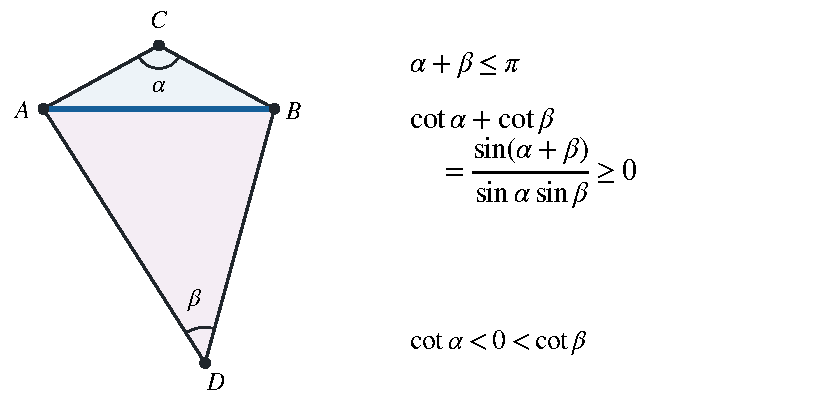
\includegraphics[width=.85\linewidth]{paired_cotangents.pdf}
\caption{For an edge $e$, weak Delaunay geometry gives
$\alpha_e+\beta_e\leq\pi$ and hence
$\cot\alpha_e+\cot\beta_e\geq0$. The replacement of $|e|^2$ by its
color weight is made after this pairing. Either cotangent separately
may be negative.}
\label{fig:cotangent}
\end{figure}

\begin{theorem}[Periodic density bound]
\label{thm:periodic}
Let $L>0$. If an admissible configuration is $L\Z^2$-periodic and has $V$ point
orbits, then
\begin{equation}
\label{eq:periodic-bound}
V\leq L^2.
\end{equation}
\end{theorem}

\begin{proof}
The empty configuration is immediate. Otherwise use
Proposition~\ref{prop:triangulation}. For an edge $e=[p,q]$, set
$w_e=\omega(c(p),c(q))$. This weight is unchanged by lattice
translations, and admissibility gives $|e|^2\geq w_e$.

The incidence pairing in the proposition justifies the following finite
sums, all taken over face or edge orbits with their incidence
multiplicities:
\begin{align}
4L^2
&=4\sum_f K_f\notag\\
&=\sum_e |e|^2(\cot\alpha_e+\cot\beta_e)
\label{eq:global-lengths}\\
&\geq\sum_e w_e(\cot\alpha_e+\cot\beta_e)
\label{eq:global-weights}\\
&=\sum_f\sum_{e\subset f}w_e\cot\theta_{f,e}
\label{eq:global-faces}\\
&\geq 2F=4V.
\label{eq:global-budget}
\end{align}
The equality \eqref{eq:global-lengths} follows from
Lemma~\ref{lem:area-identity}. The only sign needed to pass to
\eqref{eq:global-weights} is the paired nonnegativity from
Lemma~\ref{lem:paired-sign}. The final inequality is the sum of
Theorem~\ref{thm:triangle} over all faces. 

In particular, the difference between the two edge sums is exactly
\[
\sum_e (|e|^2-w_e)(\cot\alpha_e+\cot\beta_e)\geq0.
\]
Each summand is nonnegative because both factors are nonnegative.
This explains why no sign assumption on an individual cotangent is
needed. If the two sides of a quotient edge belong to the same face
orbit, they are still counted as two incidences; the argument and the
inequality are unchanged.
Dividing by $4$ proves the claim.
\end{proof}

\section{Removing periodicity}
\label{sec:periodization}

We now pass from the periodic bound to arbitrary configurations. We first
find a finite square patch and remove a boundary strip so that points in
different copies of the remaining patch satisfy all separation
constraints. We can then apply the periodic theorem. All boundary losses
will be explicit. The number of points lost near the square's boundary
grows at most linearly with its side length, whereas its area grows
quadratically. This makes the loss negligible in large patches.

\begin{lemma}[A dense square]
\label{lem:dense-square}
For every admissible $C$, every $r\geq0$, and every $u>0$, there is a
half-open square of side $u$ containing a set
$T\subset C\cap\overline B(0,r)$ such that
\begin{equation}
\label{eq:dense-square}
N_C(r)u^2\leq |T|\pi(r+2u)^2.
\end{equation}
\end{lemma}

\begin{proof}
If $N_C(r)=0$, any square and $T=\varnothing$ satisfy the conclusion.
Suppose therefore that $N_C(r)>0$. Partition the plane into the
half-open squares
\[
Q_{m,n}=[mu,(m+1)u)\times[nu,(n+1)u),
\qquad(m,n)\in\Z^2.
\]
Each point belongs to exactly one square. Let $I$ be the family of squares
containing at least one point of $C\cap\overline B(0,r)$. This family
is nonempty and finite because that point set is nonempty and finite.

For $Q\in I$, choose $p\in Q\cap C\cap\overline B(0,r)$. Every $z\in Q$
satisfies
\[
|z|\leq|p|+|z-p|\leq r+\sqrt2u\leq r+2u.
\]
Consequently the union of the squares in $I$ lies in
$\overline B(0,r+2u)$. The squares are pairwise disjoint and each has
area $u^2$, so
\[
|I|u^2\leq\pi(r+2u)^2.
\]
Choose a square $Q_*$ maximizing
$\#(Q\cap C\cap\overline B(0,r))$ over $Q\in I$, and put
$T=Q_*\cap C\cap\overline B(0,r)$. Counting the points square by square
gives
\[
N_C(r)=\sum_{Q\in I}\#(Q\cap C\cap\overline B(0,r))
\leq |I||T|.
\]
Multiplying by $u^2$ and using the area bound proves
\eqref{eq:dense-square}.
\end{proof}

\begin{lemma}[Points in a rectangle]
\label{lem:rectangle}
If a finite $1$-separated set $D$ lies in a rectangle of width $w\geq0$
and height $h\geq0$, then
\begin{equation}
\label{eq:rectangle}
|D|\frac\pi4\leq(w+1)(h+1).
\end{equation}
\end{lemma}

\begin{proof}
The open disks of radius $1/2$ centered at distinct points of $D$ are
disjoint: a point in two such disks would, by the triangle inequality,
give a distance less than $1$ between their centers. Each disk has area
$\pi/4$, and all these disks lie in the rectangle enlarged by $1/2$
on each of its four sides. The enlarged rectangle has width $w+1$ and
height $h+1$. Comparing areas gives \eqref{eq:rectangle}, including when
$w=0$ or $h=0$.
\end{proof}

Let the square in Lemma~\ref{lem:dense-square} be
$[a,a+u)\times[b,b+u)$, where $u\geq2$. Delete its boundary strip of
width $1$ by setting
\begin{equation}
\label{eq:interior-patch}
S=T\cap\bigl([a+1,a+u-1]\times[b+1,b+u-1]\bigr).
\end{equation}
The set $T\setminus S$ is contained in the union of the four closed
rectangles
\[
\begin{split}
&[a,a+1]\times[b,b+u],\qquad
 [a+u-1,a+u]\times[b,b+u],\\
&[a,a+u]\times[b,b+1],\qquad
 [a,a+u]\times[b+u-1,b+u].
\end{split}
\]
Two have dimensions $1\times u$ and two have dimensions $u\times1$.
The points in each are $1$-separated, so Lemma~\ref{lem:rectangle}
bounds their number by $8(u+1)/\pi$. Adding these four estimates may
count corner points more than once, which only increases the bound.
Since $\pi>3$ and $32/3<11$, we obtain
\[
|T\setminus S|\leq\frac{32}{\pi}(u+1)<11(u+1).
\]
In particular,
\begin{equation}
\label{eq:boundary-loss}
|T|\leq |S|+11(u+1).
\end{equation}
The argument also applies at $u=2$, when the retained square can
degenerate to a single point.

\begin{lemma}[Buffered periodization]
\label{lem:periodization}
For $u\geq2$, the coloring of $S$ extends $u\Z^2$-periodically to an
admissible configuration $S+u\Z^2$, with precisely $|S|$ point orbits.
\end{lemma}

\begin{proof}
If $S=\varnothing$, all assertions are immediate. Otherwise assign to
the point $s+uk$, where $s\in S$ and $k\in\Z^2$, the color of $s$.
We first check that different copies cannot meet or create a forbidden
distance. After subtracting a common translation, two points in
different copies have the form $s$ and $t+u(m,n)$, with $s,t\in S$
and $(m,n)\ne(0,0)$. If $m\ne0$, then
\eqref{eq:interior-patch} gives $|s_1-t_1|\leq u-2$, and hence
\[
|s_1-(t_1+um)|
\geq u|m|-|s_1-t_1|
\geq u-(u-2)=2.
\]
If $m=0$, then $n\ne0$ and the same calculation in the second
coordinate gives distance at least $2$. Thus points from different
copies cannot coincide. Their Euclidean distance is at least $2$, so
its square is at least $4$, whereas every color weight is at most $2$.

Within one copy, distinct points have exactly their original distances
and colors, and therefore inherit admissibility from $C$. The preceding
noncoincidence also shows that every point has a unique representation
as $s+uk$. Thus the coloring is well defined and periodic. Finally,
if $s,t\in S$ belong to the same $u\Z^2$-orbit, a nonzero translation
between them would contradict the distance estimate. They must be
equal. Hence there are exactly $|S|$ point orbits.
\end{proof}

Theorem~\ref{thm:periodic} and Lemma~\ref{lem:periodization} now give
\begin{equation}
\label{eq:patch-periodic-bound}
|S|\leq u^2.
\end{equation}
Combining \eqref{eq:dense-square}, \eqref{eq:boundary-loss}, and
\eqref{eq:patch-periodic-bound} gives a quantitative form of the theorem.

\begin{proposition}
\label{prop:quantitative}
For every admissible configuration and every $r\geq4$,
\begin{equation}
\label{eq:quantitative-density}
\frac{N_C(r)}{\pi r^2}
\leq1+\frac{15}{\sqrt r}+\frac{59}{r}
       +\frac{88}{r^{3/2}}+\frac{44}{r^2}.
\end{equation}
\end{proposition}

\begin{proof}
The square side must grow to reduce the relative boundary loss, while
remaining small compared with the disk radius. Choose $u=\sqrt r\geq2$.
The three preceding estimates yield
\[
N_C(r)u^2
\leq |T|\pi(r+2u)^2
\leq\bigl(u^2+11u+11\bigr)\pi(r+2u)^2.
\]
Dividing by the positive quantity $\pi r^2u^2$ and using $r=u^2$
gives
\[
\frac{N_C(r)}{\pi r^2}
\leq\left(1+\frac{11}{u}+\frac{11}{u^2}\right)
     \left(1+\frac{2}{u}\right)^2.
\]
Expanding the product gives
\begin{align*}
1+\frac{4+11}{u}
 +\frac{4+44+11}{u^2}
 +\frac{44+44}{u^3}
 +\frac{44}{u^4}
&=1+\frac{15}{u}+\frac{59}{u^2}
    +\frac{88}{u^3}+\frac{44}{u^4}.
\end{align*}
Substituting $u=\sqrt r$ proves \eqref{eq:quantitative-density}.
\end{proof}

\begin{proof}[Proof of the density assertion in Theorem~\ref{thm:main}]
For $r\geq1$, each of $r^{-1}$, $r^{-3/2}$, and $r^{-2}$ is at most
$r^{-1/2}$. Since $15+59+88+44=206$, \eqref{eq:quantitative-density}
implies
\[
\frac{N_C(r)}{\pi r^2}\leq1+\frac{206}{\sqrt r}
\qquad(r\geq4).
\]
Given $\varepsilon>0$, choose
\[
R_\varepsilon=\max\left\{4,\left(\frac{206}{\varepsilon}\right)^2\right\}.
\]
For every $r\geq R_\varepsilon$, we have $206/\sqrt r\leq\varepsilon$.
This proves \eqref{eq:main-eventual} with an explicit radius independent
of the configuration. Taking the upper limit and then letting
$\varepsilon\downarrow0$ proves \eqref{eq:main-limsup}.

The equivalence of the two formulations does not require an ordinary
density limit. The disjoint open disks of radius $1/2$
centered at points counted by $N_C(r)$ lie in $B(0,r+1/2)$, so
\[
N_C(r)\frac\pi4\leq\pi(r+1/2)^2,
\qquad
N_C(r)\leq4(r+1/2)^2\leq9r^2\quad(r\geq1).
\]
Therefore $g(r)=N_C(r)/(\pi r^2)$ is a bounded real-valued function on
$[1,\infty)$. Its upper limit is
\[
\limsup_{r\to\infty}g(r)
=\inf_{R\geq1}\sup_{r\geq R}g(r).
\]
If this infimum is at most $1$, then for each $\varepsilon>0$ some
$R\geq1$ has $\sup_{r\geq R}g(r)<1+\varepsilon$, which implies
\eqref{eq:main-eventual}. Conversely, \eqref{eq:main-eventual} bounds
the displayed infimum by $1+\varepsilon$ for every $\varepsilon>0$,
and hence by $1$. This establishes the asserted equivalence.
\end{proof}

\section{Sharpness}
\label{sec:sharpness}

Take $C=\Z^2$ with the checkerboard coloring
\begin{equation}
\label{eq:checkerboard}
c(m,n)=
\begin{cases}
0,&m+n\text{ even},\\
2,&m+n\text{ odd}.
\end{cases}
\end{equation}
For two points of the same color, their difference is a nonzero
integer vector with even coordinate sum. Its squared length is a positive
integer. Squared length $1$ is possible only for $(\pm1,0)$ or
$(0,\pm1)$, all of which have odd coordinate sum. Thus the squared
length for equal colors is at least $2$. For opposite colors, the
nonzero integer difference has squared length at least $1$. No adjacent
colors occur in this coloring, so those conditions are vacuous. This
verifies every admissibility condition.

To compute the density, put $b=1/\sqrt2$ and let
\[
Q_z=z+[-1/2,1/2)^2\qquad(z\in\Z^2).
\]
These half-open unit squares partition the plane, and every point of
$Q_z$ is at distance at most $b$ from $z$. For $r\geq b$, set
$W_r=\bigcup_{|z|\leq r}Q_z$. If $y\in W_r$, the triangle inequality
gives $|y|\leq r+b$. Conversely, if $|y|\leq r-b$, choose the unique
square $Q_z$ containing $y$. Then $|z|\leq|y|+|z-y|\leq r$, so
$y\in W_r$. Consequently
\[
\overline B(0,r-b)\subset W_r\subset\overline B(0,r+b).
\]
The squares in $W_r$ are disjoint and each has area $1$. Taking areas
therefore gives
\[
\pi(r-1/\sqrt2)^2
\leq N_{\Z^2}(r)
\leq\pi(r+1/\sqrt2)^2.
\]
Dividing by $\pi r^2$ gives the lower and upper bounds
$(1\mp1/(\sqrt2 r))^2$, respectively. Both tend to $1$, so the squeeze
theorem yields
\[
\lim_{r\to\infty}\frac{N_{\Z^2}(r)}{\pi r^2}=1.
\]
This proves sharpness in Theorem~\ref{thm:main}. Appendix~\ref{app:density}
shows that \eqref{eq:checkerboard} yields $D_5$ under the fiber
construction.

The two triangle families in Theorem~\ref{thm:triangle} classify equality
in the local inequality. They do not by themselves classify all global
configurations of density $1$: local equality and asymptotic equality
are different assertions. For example, removing one point from the
checkerboard configuration preserves admissibility and its limiting
density. We make no classification of all density-$1$ configurations.

This completes the proof of Theorem~\ref{thm:main}: every admissible
configuration has upper density at most $1$, and this bound is attained.
In particular, Conjecture~4.1 of Cohn and Rajagopal is proved. The
remaining sections discuss the five-dimensional consequence and the scope
of formal verification.

\section{The fibered packing consequence}
\label{sec:fibers}

We recall the construction of Cohn and Rajagopal~\cite[Section~4.1]{CR}.
Let
\[
D_3=\{x\in\Z^3:x_1+x_2+x_3\equiv0\pmod2\}.
\]
Its covolume (the volume of a fundamental cell) is $2$, and its minimum
nonzero length is $\sqrt2$. The dual lattice $D_3^*$ consists of vectors
whose inner product with every vector of $D_3$ is an integer. Two shifts
in $D_3^*$ give the same translate of $D_3$ exactly when their difference
lies in $D_3$. There are four resulting classes, cyclically indexed by
$\Z/4\Z$, with representatives
\begin{equation}
\label{eq:coset-representatives}
t_0=(0,0,0),\quad
t_1=\tfrac12(1,1,1),\quad
t_2=(0,0,1),\quad
t_3=\tfrac12(1,1,-1).
\end{equation}
A point $p$ of the planar base specifies the first two coordinates of
a fiber of centers. Its color selects the translated lattice
$D_3+t_{c(p)}$ for the last three coordinates. Translation preserves all
distances within a fiber. The minimum distance between the translates
$D_3+t_i$ and $D_3+t_j$ is $0$, $\sqrt3/2$, or $1$ according as the
colors are equal, adjacent, or opposite. Consequently
\begin{equation}
\label{eq:fiber-centers}
X_C=\bigcup_{p\in C}\bigl(\{p\}\times(D_3+t_{c(p)})\bigr)
\subset\R^2\times\R^3
\end{equation}
is a packing center set for balls of radius $a=1/\sqrt2$ exactly when
$(C,c)$ is admissible. Within a fiber, the minimum distance is already
$2a=\sqrt2$. Between fibers, squared distances in the two orthogonal
factors add. Subtracting the squared minimum distances $0$, $3/4$, and
$1$ in the last three coordinates from $2$ gives the planar thresholds
$2$, $5/4$, and $1$.

Point density counts centers per unit volume; packing density measures
the fraction of volume occupied by the balls. For a center set
$P\subset\R^5$ as above, define its upper packing density by
\[
\overline\delta(P)=
\limsup_{R\to\infty}
\frac{\vol\bigl(U_a(P)\cap\overline B_5(0,R)\bigr)}
     {\vol\bigl(\overline B_5(0,R)\bigr)},
\qquad
U_a(P)=\bigcup_{x\in P}\overline B_5(x,a).
\]

\begin{corollary}
\label{cor:fiber-density}
Every admissible configuration gives a packing \eqref{eq:fiber-centers}
whose upper packing density is at most
\begin{equation}
\label{eq:d5-density}
\frac{\pi^2\sqrt2}{30}.
\end{equation}
This bound is attained by $D_5$.
\end{corollary}

For a periodic base of point density $\delta$, the packing density is
$\delta\pi^2\sqrt2/30$, as follows by multiplying the base density,
the fiber center density $1/2$, and the ball volume
$\pi^2\sqrt2/15$; see~\cite[Section~4.1]{CR}.
For completeness, Appendix~\ref{app:density} proves the corollary
without assuming periodicity or an ordinary density limit for the base.
The conclusion concerns only this four-coset $D_3$-fibered family.

\appendix

\section{The five-dimensional density transfer}
\label{app:density}

We justify Corollary~\ref{cor:fiber-density} for arbitrary admissible
bases. Write $\kappa_d$ for the volume of the unit ball in $\R^d$;
thus $\kappa_3=4\pi/3$ and $\kappa_5=8\pi^2/15$.

\paragraph{Counting centers.}
Choose a bounded half-open fundamental parallelepiped $F$ for $D_3$
with $\vol(F)=2$ and $F\subset\overline B_3(0,\rho)$.
For each coset $D_3+t_i$, the cells $y+F$ partition $\R^3$.
Those with $|y|\leq s$ lie in $\overline B_3(0,s+\rho)$, so
\begin{equation}
\label{eq:lattice-cell-bound}
\#\bigl((D_3+t_i)\cap\overline B_3(0,s)\bigr)
\leq\frac{\kappa_3}{2}(s+\rho)^3
=\frac{\kappa_3}{2}s^3+O(s^2+1)
\qquad(s\geq0).
\end{equation}
The error comes from the cells near the boundary of the ball, and its
implied constant is uniform in the four cosets.
Put $N_{X_C}(R)=\#(X_C\cap\overline B_5(0,R))$ and
$s_p=(R^2-|p|^2)^{1/2}$ for $|p|\leq R$.
Counting each fiber in its three-dimensional section gives
\begin{equation}
\label{eq:fiber-count}
N_{X_C}(R)
\leq\frac{\kappa_3}{2}
\sum_{\substack{p\in C\\|p|\leq R}}s_p^3+O(R^4).
\end{equation}
Indeed, $s_p\leq R$ and separation gives
$N_C(R)\leq4(R+1/2)^2=O(R^2)$, so the sum of the errors in
\eqref{eq:lattice-cell-bound} is $O(R^4)$ for $R\geq1$.

It remains to bound the weighted sum of section volumes in
\eqref{eq:fiber-count}. We express it using the planar counting function,
to which Theorem~\ref{thm:main} applies. Fix $\varepsilon>0$.
The theorem and local finiteness give
a constant $M_\varepsilon\geq0$ such that
\begin{equation}
\label{eq:radial-bound-with-constant}
N_C(r)\leq(1+\varepsilon)\pi r^2+M_\varepsilon
\qquad(r\geq0).
\end{equation}
For example, choose $R_0$ beyond which the theorem's eventual bound
holds and take $M_\varepsilon=N_C(R_0)$.
Writing
$(R^2-|p|^2)^{3/2}=\int_{|p|}^R3r\sqrt{R^2-r^2}\,dr$
and interchanging the finite sum and integral yields
\begin{equation}
\label{eq:radial-integral}
\sum_{\substack{p\in C\\|p|\leq R}}s_p^3
=\int_0^R3r\sqrt{R^2-r^2}\,N_C(r)\,dr.
\end{equation}
The factor $3r\sqrt{R^2-r^2}$ is nonnegative for $0\leq r\leq R$.
We may therefore substitute \eqref{eq:radial-bound-with-constant}
into the integral to obtain
\begin{equation}
\label{eq:weighted-base-bound}
\sum_{\substack{p\in C\\|p|\leq R}}s_p^3
\leq(1+\varepsilon)\frac{\kappa_5}{\kappa_3}R^5
     +M_\varepsilon R^3.
\end{equation}
Here
$\int_0^R3\pi r^3\sqrt{R^2-r^2}\,dr
=(2\pi/5)R^5=(\kappa_5/\kappa_3)R^5$ and
$\int_0^R3r\sqrt{R^2-r^2}\,dr=R^3$.
Combining \eqref{eq:fiber-count} and \eqref{eq:weighted-base-bound},
dividing by $\kappa_5R^5$, and taking the upper limit with
$\varepsilon$ fixed gives a bound of $(1+\varepsilon)/2$.
Letting $\varepsilon\downarrow0$, we obtain
\begin{equation}
\label{eq:center-density}
\limsup_{R\to\infty}\frac{N_{X_C}(R)}{\kappa_5R^5}\leq\frac12.
\end{equation}
No ordinary density limit of the base was used.

\paragraph{Occupied volume and equality.}
A packed ball of radius $a=1/\sqrt2$ meeting $\overline B_5(0,R)$
has its center in $\overline B_5(0,R+a)$. Thus
\[
\vol\bigl(U_a(X_C)\cap\overline B_5(0,R)\bigr)
\leq\kappa_5a^5N_{X_C}(R+a).
\]
Divide by $\kappa_5R^5$ and use \eqref{eq:center-density} and
$(R+a)^5/R^5\to1$ to obtain
\[
\overline\delta(X_C)\leq\frac12\kappa_5a^5
=\frac{\pi^2\sqrt2}{30}.
\]

For the checkerboard coloring \eqref{eq:checkerboard}, the fiber
over $(m,n)$ is $D_3$ for even $m+n$ and $D_3+(0,0,1)$ for odd
$m+n$. Therefore
\[
X_C=\{x\in\Z^5:x_1+\cdots+x_5\equiv0\pmod2\}=D_5.
\]
This is an index-$2$ sublattice of $\Z^5$, so its covolume is $2$.
Comparing its bounded fundamental cells with balls of radii
$R\pm\sigma$, for a fixed cell bound $\sigma$, gives
$N_{D_5}(R)=(\kappa_5/2)R^5+O(R^4)$.
For $R>a$, the occupied volume is bounded on both sides by
\[
\kappa_5a^5N_{D_5}(R-a)
\leq\vol\bigl(U_a(D_5)\cap\overline B_5(0,R)\bigr)
\leq\kappa_5a^5N_{D_5}(R+a).
\]
The lower bound uses disjoint interiors; only finitely many packed
balls meet each bounded window, and their boundaries have zero volume.
After division by $\kappa_5R^5$, both bounds tend to
$\kappa_5a^5/2=\pi^2\sqrt2/30$. This proves attainment and completes
the proof of Corollary~\ref{cor:fiber-density}.

\section{Formal verification status}
\label{app:formal}

A supplementary source archive provides a formal development in
Lean 4~\cite{Lean4} with Mathlib~\cite{Mathlib}.

The supplementary project \texttt{Conjecture41\_Lean} formalizes the
upper-density bound in Theorem~\ref{thm:main}, in the literal formulation
of Conjecture~4.1.

The theorem \texttt{Audit41.published\_statement} gives the result in
the notation of the original conjecture. Its hypotheses are an arbitrary
planar set, a coloring defined on that set, and the three original
distance bounds. Its conclusions are local finiteness and the upper
radial point-density bound in \eqref{eq:main-limsup}.

The underlying declarations
\texttt{conjecture\_4\_1} and \texttt{conjecture\_4\_1\_limsup}
in namespace \texttt{Conjecture41} give the eventual bound and the
real-valued limsup; the required boundedness is proved.

The formalization does not cover the local equality classification in
Theorem~\ref{thm:triangle}, the explicit finite-radius coefficients in
Proposition~\ref{prop:quantitative}, the sharpness example in
Section~\ref{sec:sharpness}, or the five-dimensional density transfer and
$D_5$ identification in Appendix~\ref{app:density}.
These have paper proofs. Bibliographic and historical-priority claims
are also outside the formal scope.

The supplementary material is a standalone source project. Running \texttt{./build.sh}
from its extracted root obtains the pinned Lean and Mathlib dependencies, compiles
all local proof modules, and checks the final declarations and their
transitive axiom dependencies. The normal default build includes
\texttt{Audit41.published\_statement} and the final axiom guards.
The guards accept only
\texttt{propext}, \texttt{Classical.choice}, and \texttt{Quot.sound};
an additional axiom or admitted proof in these dependencies makes
verification fail.
The archive README specifies prerequisites and exact dependency versions;
the script records its outcome in \texttt{build-logs/}.

\paragraph{Use of AI tools.}
Aristotle and ChatGPT were used to assist with checking the Lean
formalization. AI tools were also used for editorial assistance.
The formal verification described above is performed by Lean's kernel.

\section*{Acknowledgments}
We thank Henry Cohn for his interest in this work and his encouraging
comments on an early version of the manuscript. We are also grateful for
his helpful correspondence and suggestions concerning related questions
in five-dimensional sphere packing.

\begin{thebibliography}{9}
\raggedright

\bibitem{CR}
H. Cohn and I. Rajagopal,
\emph{Variations on five-dimensional sphere packings},
Discrete \& Computational Geometry (2026), published online 4 July 2026.
\href{https://doi.org/10.1007/s00454-026-00841-x}{doi:10.1007/s00454-026-00841-x}.
Also available as arXiv:2412.00937v3.
\url{https://arxiv.org/abs/2412.00937v3}.

\bibitem{Salmon}
A. Salmon,
\emph{Linear programming bounds for fibered sphere packings},
arXiv:2607.25254v1 (2026).
\url{https://arxiv.org/abs/2607.25254v1}.

\bibitem{BS}
A. I. Bobenko and B. A. Springborn,
\emph{A discrete Laplace--Beltrami operator for simplicial surfaces},
Discrete \& Computational Geometry \textbf{38} (2007), 740--756.
\href{https://doi.org/10.1007/s00454-007-9006-1}{doi:10.1007/s00454-007-9006-1}.

\bibitem{Lean4}
L. de Moura and S. Ullrich,
\emph{The Lean 4 theorem prover and programming language},
in Automated Deduction---CADE 28,
Lecture Notes in Computer Science \textbf{12699}, Springer, 2021,
625--635.
\href{https://doi.org/10.1007/978-3-030-79876-5_37}{doi:10.1007/978-3-030-79876-5\_37}.

\bibitem{Mathlib}
The mathlib Community,
\emph{The Lean mathematical library},
in Proceedings of the 9th ACM SIGPLAN International Conference on
Certified Programs and Proofs (CPP 2020), ACM, 2020, 367--381.
\href{https://doi.org/10.1145/3372885.3373824}{doi:10.1145/3372885.3373824}.
arXiv:1910.09336.

\end{thebibliography}

\end{document}
